\section{GAN for Time Series}


\begin{frame}{ForGAN architecture for time series probability forecasting}
   
To generate the future probability distribution of a time series $c = x_0, x_1, \ldots, x_t$, the following steps are taken:
\begin{enumerate}
    \item Train generator and discriminator using the CGAN or CWGAN loss function using $c_{[t_0, t]}$ as condition and $x_{t+1}$ as target.
    \item The generator is run multiple times using the same trajectory $c$ but perturbed noise vector $z$ obtaining an empirical distribution.
\end{enumerate}

\begin{figure}[H]
    \centering
    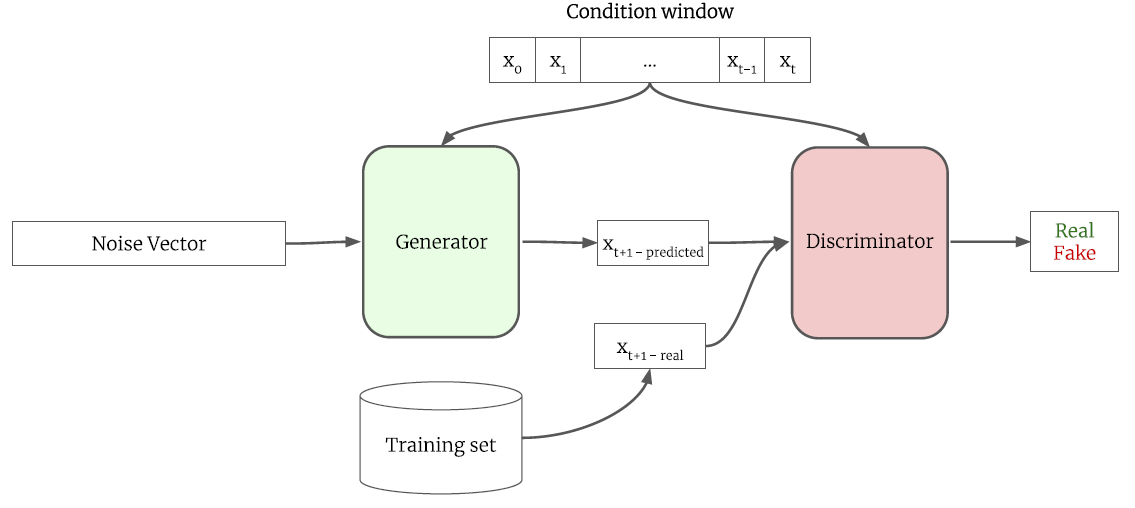
\includegraphics[scale=0.4]{images/forgan.png}
\end{figure}

\end{frame}


\begin{frame}{ForGAN architecture for time series probability forecasting}
\begin{columns}[c]

    \begin{column}{0.38\textwidth}

        \textbf{Generator}

        \vspace{0.1cm}

        It receives:
        \begin{itemize}
            \item conditioning information $c$ processed by a RNN that outputs a hidden state $h$
            \item latent noise $z$
            \item $z$ and $h$ are concatenated and processed by a FFN and outputs the next time step $x_{t+1}$
        \end{itemize}


        \textbf{Discriminator/Critic}

        \vspace{0.1cm}

        It receives the concatenated $(c, x_{t+1})$ 
        which is processed by a RNN. The hidden state $h$ is then processed by a FFN to output 
        the probability/score of the sample being real or fake.

    \end{column}

    \begin{column}{0.58\textwidth}

        \centering
        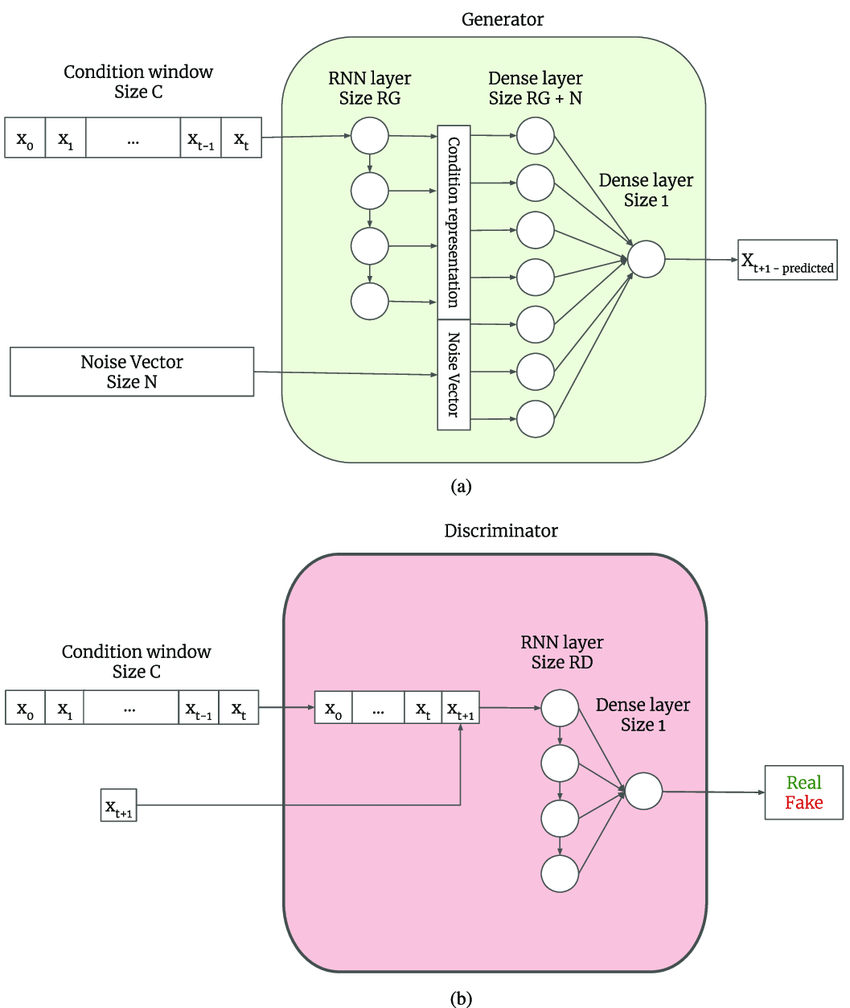
\includegraphics[height=0.82\textheight]{images/forgan_rnn.png}

    \end{column}

\end{columns}
\end{frame}

\begin{frame}{ForGAN architecture for time series probability forecasting}

The LSTM is designed to capture
\textbf{long-term dependencies} in sequential data while mitigating
the vanishing-gradient problem of standard RNNs.



\begin{equation} 
  \label{eq:imv_lstm} 
  \begin{aligned} 
& {\left[\begin{array}{c} 
\tilde{\mathbf{i}}_t \\ 
\tilde{\mathbf{f}}_t \\ 
\tilde{\mathbf{o}}_t 
\end{array}\right]=\sigma\left(\mathcal{W} \tilde{\mathbf{h}}_{t-1}+\mathcal{U} \mathbf{x}_t+\mathbf{b}\right)} \\ 
&\tilde{\mathbf j}_t=\tanh\left(\mathcal W_c\tilde{\mathbf h}_{t-1}+\mathcal U_c\mathbf x_t+\mathbf b_c\right) \\
& \tilde{\mathbf{c}}_t=\tilde{\mathbf{f}}_t \odot \tilde{\mathbf{c}}_{t-1}+\tilde{\mathbf{i}}_t \odot \tilde{\mathbf{j}}_t \qquad \text{carries long-term information}\\ 
& \tilde{\mathbf{h}}_t=\tilde{\mathbf{o}}_t \odot \tanh \left(\tilde{\mathbf{c}}_t\right) \qquad \text{carries the current sequential representation}
\end{aligned} 
\end{equation} 

\begin{figure} [H]
    \centering
    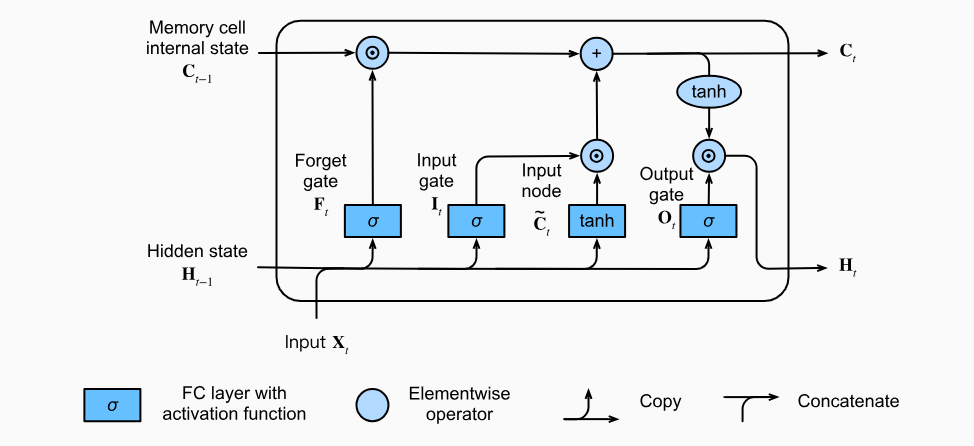
\includegraphics[scale=0.35]{images/LSTM.png}
\end{figure}
\end{frame}